\section{Introduction}
%pretrained Language models ({\lmabbr}s) have shown strong performance on various natural language processing tasks~\citep{devlin-etal-2019-bert,liu2019roberta,raffel2020exploring}, while large language models (LLMs)~\citep{brown2020language,zhang2022opt} with more parameters show their reasoning and generalization capabilities outperforming small {\lmabbr}s~\citep{kaplan2020scaling}. 
% \hanna{please dont' use PLM and LLM acronyms... just use LMs and add pretrained or large adjectives if needed.} 
% \hanna{first sentence is not needed} 
Fine-tuning language models (LMs)~\citep{devlin-etal-2019-bert,liu2019roberta,raffel2020exploring} is an essential paradigm to adapt them to downstream tasks~\citep{mishra-etal-2022-cross,wang-etal-2022-super}. Increasing the parameter scale of LMs improves model performance~\citep{kaplan2020scaling}, but incurs significant training and inference costs.  
%However, as the parameter size of {\lmabbr} increases, both training and inference efficiency bottlenecks hinder the practicality of {\lmabbr}'s wide usage. 
For instance, a 13B LLaMA model~\citep{touvron2023llama} costs about 100GB memory for fine-tuning and 30GB for inference with float16 datatype. 
It is important to improve the training and inference efficiency of {\lmabbr} for practical applications.

\begin{figure}[t!]
    \centering
    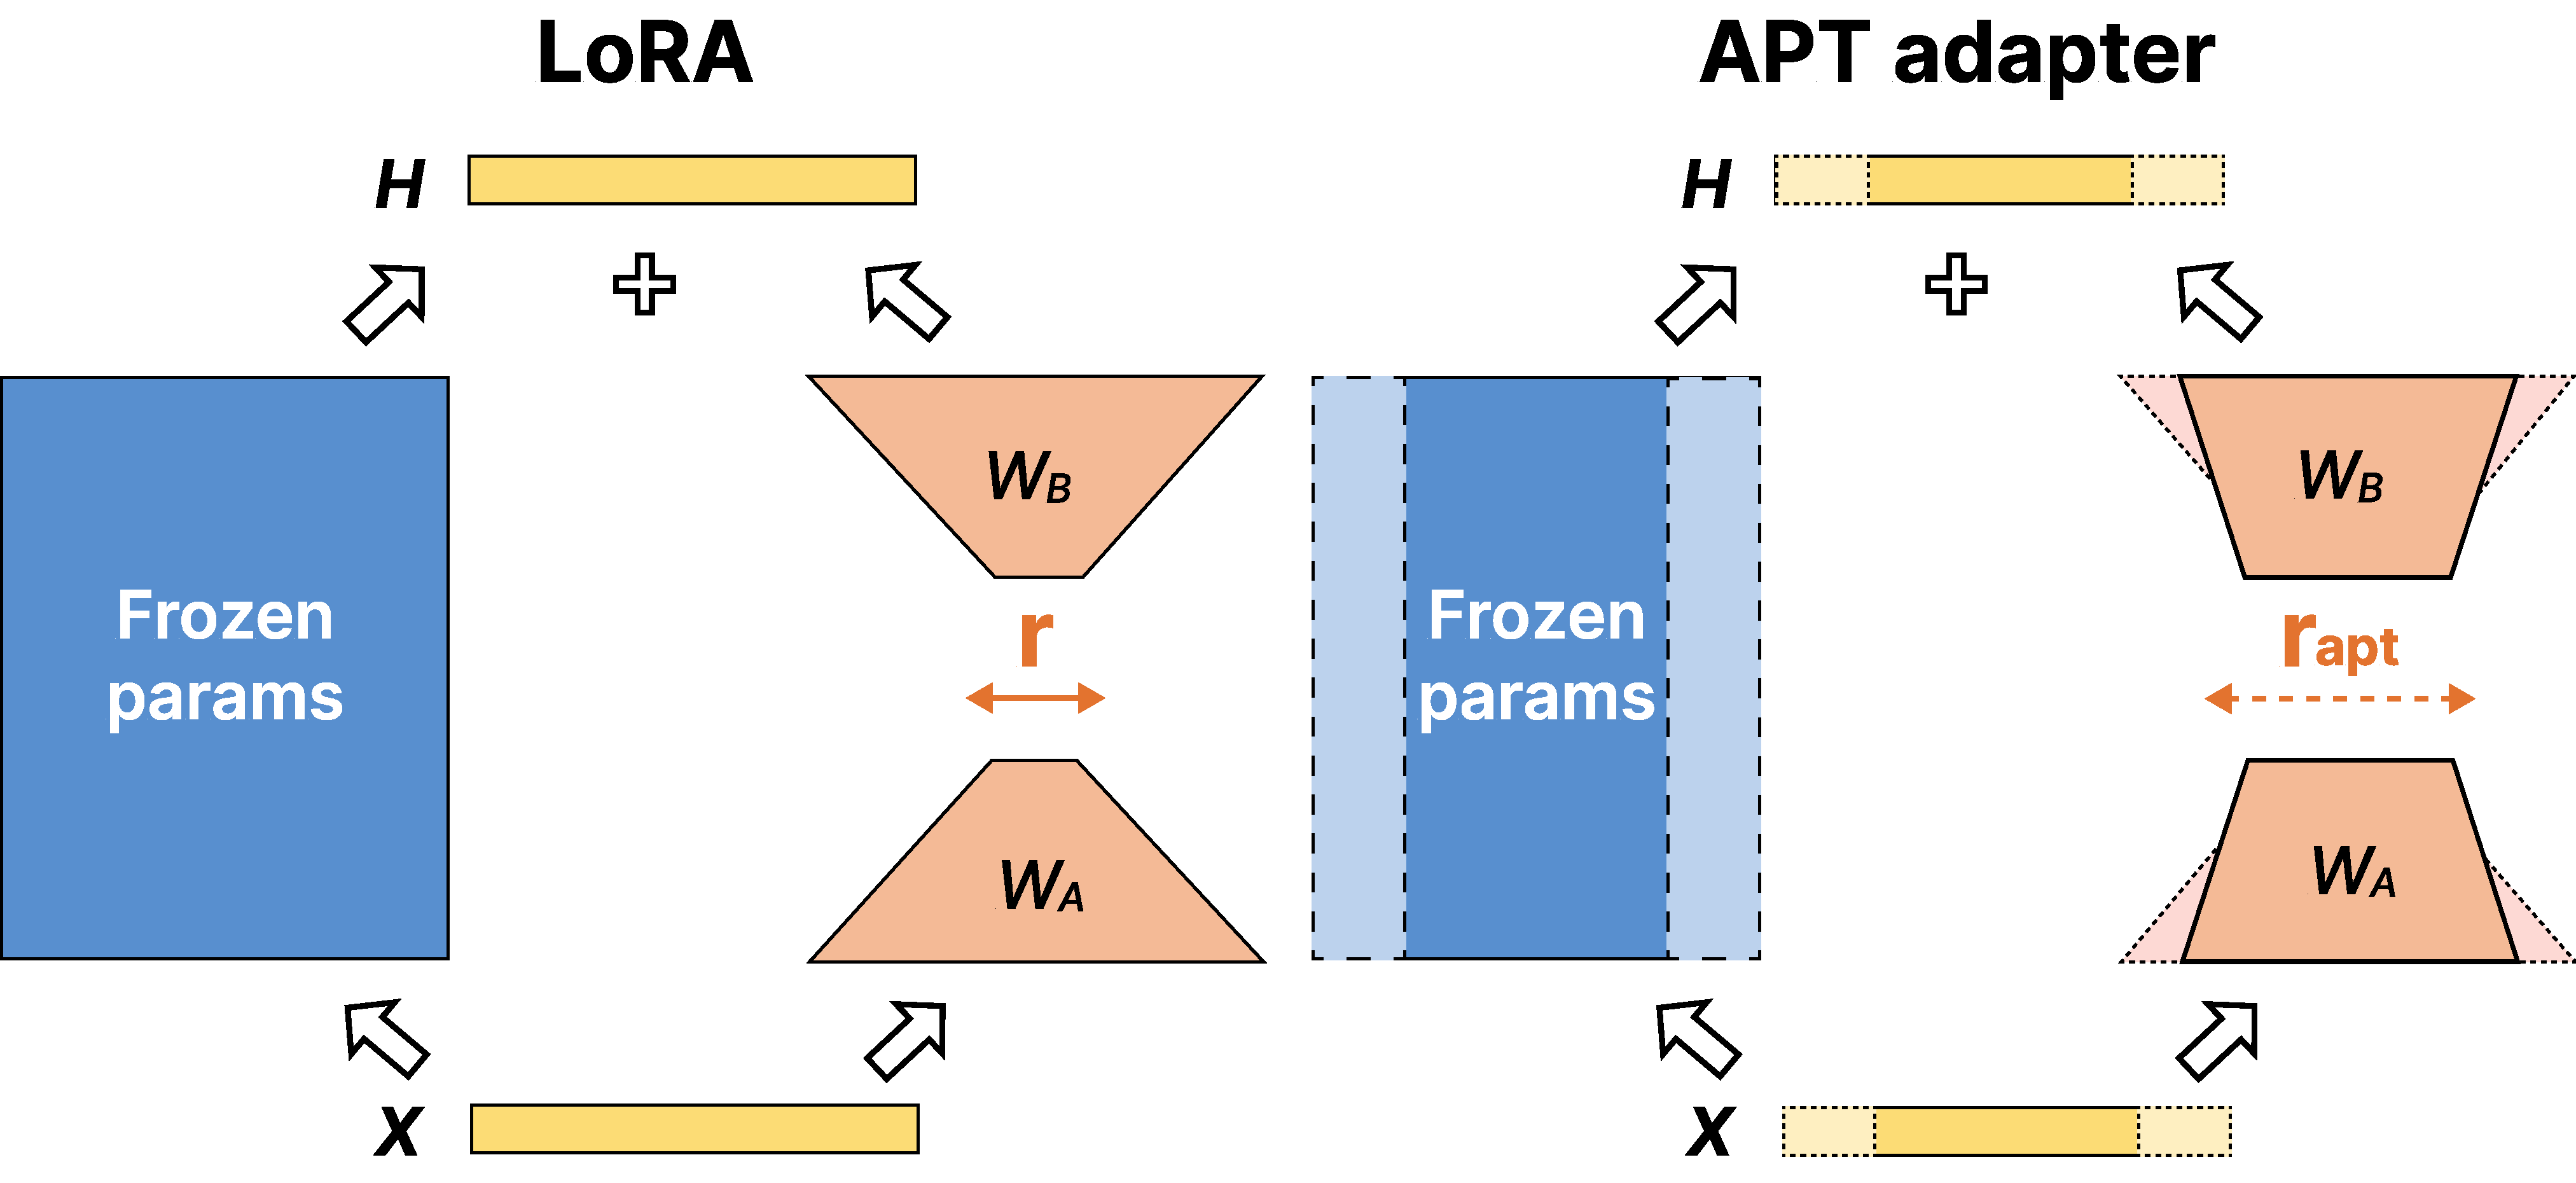
\includegraphics[width=0.9\linewidth]{figures/teaser_figure_revised.pdf}
\caption{{\ourmethod} provides both training and inference efficiency benefits by pruning and tuning pretrained LM parameters adaptively via the \textbf{{\ourmethod} adapter}. We dynamically adjust (add/reduce) {\ourmethod} adapter input/output dimensions and the rank ($r_{\text{apt}}$). Reducing adapter dimensions prunes frozen parameters, making training and inference faster and more memory-efficient. Adding adapter ranks helps recover the pruned {\lmabbr}'s task performance. In contrast, existing adapters like LoRA allow efficient training but do not provide inference efficiency since the model size is not reduced.}
    \label{fig:teaser}
    \vspace{-15pt}
\end{figure}


% \qq{We can first discuss efficient training, PEFT methods, their main benefits are memory reduction, no speedup etc. Deploying PEFT trained models do not directly provide inference efficiency, so we discuss inference efficiency methods like quantization, pruning etc. And those inference methods requires full fine-tuning, and naive solutions like applying PEFT+quant/pruning do not work out of the box. Then you describe why it does not work, and what are the challenges (you already have something about this in the next paragraph).}

% Please add the following required packages to your document preamble:
% \usepackage{booktabs}
\begin{table*}[t!]
\centering
\small
\begin{tabular}{@{}ll|cc|cc|cc@{}}
\toprule
\multicolumn{2}{l|}{\multirow{2}{*}{Method}} & \multirow{2}{*}{$\mathcal{A}_{\text{P}}$} & \multirow{2}{*}{$\mathcal{A}_{\text{T}}$} & \multicolumn{2}{c|}{Training}                                             & \multicolumn{2}{c}{Inference}                                                        \\
\multicolumn{2}{l|}{}                        &                     &                     & T                                          & M                         & T                                                  & M                          \\ \midrule
\multirow{3}{*}{PEFT}       & Adapter~\citep{Pfeiffer2020AdapterFusionNT}        & \xmark              & \xmark              & \color{red}$\Uparrow_{\text{High}}$ & \color{ForestGreen}$\Downarrow_{\text{Low}}$ & \color{red}$\Uparrow_{\text{Low}}$                              & \color{red}$\Uparrow_{\text{Low}}$      \\
                            & LoRA~\citep{hu_lora_2021}           & \xmark              & \xmark              & \color{red}$\Uparrow_{\text{High}}$ & \color{ForestGreen}$\Downarrow_{\text{Low}}$ & \textbf{=}                                         & \textbf{=}                 \\
                            & AdaLoRA~\citep{zhang2023adaptive}        & \xmark              & \cmark              & \color{red}$\Uparrow_{\text{High}}$ & \color{ForestGreen}$\Downarrow_{\text{Low}}$ & \textbf{=}                                         & \textbf{=}                 \\ \midrule
\multirow{4}{*}{Pruning}    & MvP~\citep{sanh_movement_2020}            & \xmark              & \xmark              & \color{red}$\Uparrow_{\text{High}}$ & \color{red}$\Uparrow_{\text{Low}}$     & \color{ForestGreen}$\Downarrow_{\text{Low}}$                         & \color{ForestGreen}$\Downarrow_{\text{Low}}$ \\
                            & BMP~\citep{lagunas_block_2021}            & \xmark              & \xmark              & \color{red}$\Uparrow_{\text{High}}$ & \color{red}$\Uparrow_{\text{Low}}$     & \color{ForestGreen}$\Downarrow_{\text{High}}$ & \color{ForestGreen}$\Downarrow_{\text{Low}}$  \\
                            & CoFi~\citep{xia_structured_2022}           & \xmark              & \xmark              & \color{red}$\Uparrow_{\text{High}}$ & \color{red}$\Uparrow_{\text{Low}}$     & \color{ForestGreen}$\Downarrow_{\text{High}}$ & \color{ForestGreen}$\Downarrow_{\text{Low}}$  \\
                            & MT~\citep{kwon_fast_2022}             & \xmark              & \xmark              & \textbf{=}                                 & \textbf{=}                & \color{ForestGreen}$\Downarrow_{\text{High}}$ & \color{ForestGreen}$\Downarrow_{\text{Low}}$  \\ \midrule
\multirow{3}{*}{Combined}   & SPA~\citep{hedegaard_structured_2022}            & \xmark              & \xmark              & \color{red}$\Uparrow_{\text{High}}$ & \color{red}$\Uparrow_{\text{Low}}$     & \color{ForestGreen}$\Downarrow_{\text{High}}$ & \color{ForestGreen}$\Downarrow_{\text{Low}}$  \\
                            & LRP~\citep{zhang2023pruning}            & \xmark              & \xmark              & \color{red}$\Uparrow_{\text{High}}$ & \color{ForestGreen}$\Downarrow_{\text{Low}}$ & \color{ForestGreen}$\Downarrow_{\text{High}}$ & \color{ForestGreen}$\Downarrow_{\text{Low}}$  \\
                            & \textbf{\ourmethod} (ours)   & \cmark              & \cmark              & \color{red}$\Uparrow_{\text{Low}}$                      & \color{ForestGreen}$\Downarrow_{\text{Low}}$ & \color{ForestGreen}$\Downarrow_{\text{High}}$ & \color{ForestGreen}$\Downarrow_{\text{Low}}$  \\ \bottomrule
\end{tabular}
\caption{Efficiency comparison of existing methods and APT. $\mathcal{A}_{\text{P}}$ stands for adaptive pruning and $\mathcal{A}_{\text{T}}$ for adaptive tuning, where the total and tuning parameter sizes are dynamically adjusted. We measure efficiency using training converge time, inference time (T), and peak memory (M). Symbols {\color{red}$\Uparrow$} and {\color{ForestGreen}$\Downarrow$} indicate increased and decreased costs, respectively, while \textbf{=} signifies no change in cost. The terms ``low'' and ``high'' qualify the extent of cost variations.} 
\label{tab:preliminary-summary}
\vspace{-15pt}
\end{table*}

Parameter-efficient fine-tuning methods (PEFT, summarized in \cref{tab:preliminary-summary})~\citep{houlsby2019parameter,li2021prefix} reduce the memory consumption of LM fine-tuning via updating a small number of parameters. However, PEFT models do not improve inference efficiency because the {\lmabbr} size remains the same or even increases after fine-tuning. For instance, LoRA~\citep{hu_lora_2021} tunes low-rank decomposed linear layers parallel to frozen parameters to reduce training memory but takes longer to converge~\citep{ding2023parameter}.
On the other hand, structured pruning~\cite{kwon_fast_2022,xia_structured_2022,ma2023llm} improves inference efficiency by removing blocks of parameters such as attention heads and feed-forward neurons in Transformer {\lmabbr}s, showing more inference speedup than sparse unstructured pruning methods~\citep{Han2015DeepCC,han2015learning,sanh_movement_2020}. However, training pruned {\lmabbr}s takes extra time to converge and incurs high memory, substantially diminishing LMs' accessibility in usage scenarios with limited computational resources.

Integrating structured pruning and PEFT could increase both training and inference efficiency. 
However, existing research~\citep{zhao2023cpet} indicates that combining PEFT and structured pruning, such as applying structured pruning over LoRA-tuned models, causes noticeable performance loss and extra training costs. It remains challenging to prune {\lmabbr}s accurately using limited training resources.

In this paper, we develop an efficient fine-tuning approach named {\ourmethod} that \textbf{A}daptively selects model parameters for \textbf{P}runing and fine-\textbf{T}uning. {\ourmethod} combines the benefits of PEFT and structured pruning to make fine-tuning and inference more efficient. Our intuition is that pre-trained {\lmabbr} parameters contain general knowledge, but their importance to downstream tasks varies. Therefore, we can remove the parameters irrelevant to the fine-tuning task in the early training stage. Early-removing these parameters improves training and inference efficiency while not substantially hurting model accuracy~\citep{frankle2021pruning,Shen_2022_CVPR,zhang2023emergent}. Meanwhile, continuously adding more parameters for fine-tuning can improve LM performance because task-specific skills live in a subset of {\lmabbr} parameters~\citep{wang-etal-2022-finding-skill,panigrahi2023task}. 

More specifically, {\ourmethod} learns the pruning masks via an outlier-aware salience scoring function to remove irrelevant {\lmabbr} parameter blocks and adds more tuning parameters during fine-tuning according to tuning layer importance. To make training more efficient, the salience scoring function is lightweight and causes little runtime and memory overhead. Combined with our self-distillation technique that shares teacher and student parameters, {\ourmethod} can accurately prune an {\lmabbr} with less training time and lower memory usage.
% {\ourmethod} is designed by observing these intuitions: a) 



% We design our {\ourarch} architecture in {\ourmethod} framework that can adaptively increase salient parameters to be tuned while pruning redundant or unimportant parameters based on the efficient outlier-aware salience scores derived from {\lmabbr} hidden states, letting {\lmabbr} training converge fast and accurate in low-memory settings.
% \qq{I remember you have a way to view the tuning and pruning parameters together and have a technique to decide which to prune and tune, say it specifically here, because "jointly identifies" is unclear how you do it.} \qq{this is vague, you can highlight the benefits or our methods clearly, like some speedup keep accuracy comparable etc.}
% \qq{prefer to avoid `novel', people can tell if your methods are novel or not} 
% \hanna{the name elastic.. does not matter here much. YOu need to describe the metho and explain what it does rather than we build our .. method}
% \qq{compress the two techqniues into two key ideas, briefly explain how to do it and why it can work or what benefits it brings}

% We conduct comprehensive experiments on various tasks with different {\lmabbr} backbones.
% \qq{mention our method benefits both small scale and large scale models, some key numbers like xx speedup, save xx memory etc.} \todo{Two sets of results: faster pruning small models and less memory pruning large {\lmabbr}s}
% \qq{what about other baselines, you could say the best results compared to baselines (it's not LoRA, should be lora+pruning?), also did you explain or define LoRA before (if not, better mention it when you talk about PEFT), otherwise it feels abrupt to suddenly mention LoRA}
% \qq{make it consistent between intro and abstract}
Experimental results show that {\ourmethod} prunes RoBERTa and T5 base models 8$\times$ faster than the LoRA plus pruning baseline while reaching 98.0\% performance with 2.4 $\times$ speedup and 78.1\% memory consumption during inference. When pruning large {\lmabbr}s like LLaMA, {\ourmethod} costs only 30\% memory compared to the state-of-the-art pruning method and still maintains 86.4\% performance with 70\% parameters. Our ablation study in \cref{sec:ablation} indicates the effectiveness of adaptive pruning and tuning. It also demonstrates that efficient distillation with {\ourarchabbr} substantially recovers small {\lmabbr}s' performance while outlier-aware salience scoring prunes large {\lmabbr}s more accurately. Our analysis in \cref{sec:analysis} demonstrates that controlled adaptive tuning with early pruning during fine-tuning improves {\lmabbr} end-task accuracy better with less training time and memory costs.
% \qq{also need to add a few key ablation results, showing that each of the proposed methods works effectively either improving efficiency or maintaining accuracy etc.}